\pagestyle{empty}
\frontmatter

%frontispiece
%\begin{figure*}[p]
%  	\centering
%  	\includegraphics[scale=0.2]{Durer/Albrecht_Dürer_The_Third_Knot.jpg}
%  	\caption{}
%  \end{figure*}
%\clearpage

\titleGM

\clearpage

%COPYRIGHT PAGE
\begin{vplace}[2]
\noindent
THE REVELATION OF JESUS CHRIST: \\READING IN LIGHT OF THE SHADOWS\\
\newline
Copyright \copyright 2022 by Caleb George\\
All rights reserved.\\
\newline
Printed in United States of America\\
\newline
Thank you for buying an authorized edition of this book and for complying with copyright laws by not reproducing, scanning, or distributing any part of it in any form without permission.
\newline
\newline
First Edition: March 2022
\newline
\newline
Kephali Press
\newline
Athens, AL 35613
\end{vplace}

\clearpage
\clearpage

\dedication
\clearpage

\ClearShipoutPicture
\AddToShipoutPicture{%
   \checkoddpage
   \transparent{0.1}
   \ifoddpage
     \put(0,0){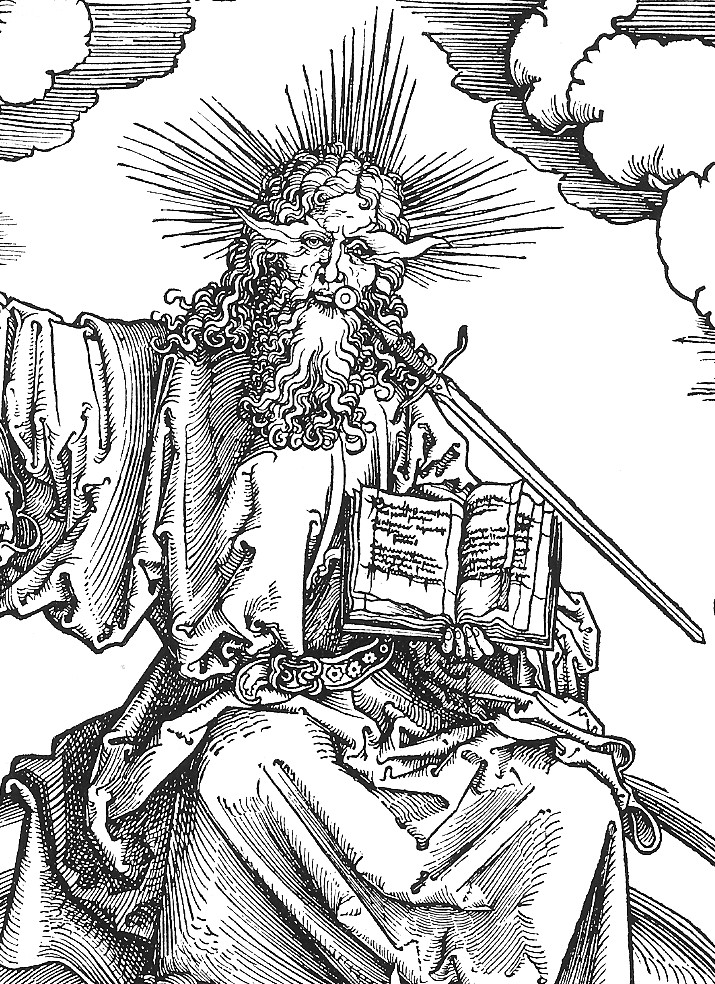
\includegraphics[width=\paperwidth,height=\paperheight]{Durer/Son_of_Man.jpg}}
   \else
     \put(0,0){\includegraphics[width=\paperwidth,height=\paperheight]{Durer/Dürer_Apocalypse_dragon.jpg}}
   \fi
}

\blankpage
\clearpage
\clearpage

\begin{KeepFromToc}
\tableofcontents
\end{KeepFromToc}
\clearpage
\listoffigures
\clearpage

%PREFACE
\chapter{Preface}
There are two things which I and many others have found to be most helpful in studying the book of Revelation: (1) Visualize the terrifying and wonderful things that Jesus showed John and (2) study the connections between the Apocalypse and the relevant Old Testament texts. This book is meant to aid in both endeavors, but especially the latter. \\

The Apocalypse is overflowing with citations and allusions to the Hebrew Bible. The Nestle-Aland 28\textsuperscript{th} edition of the Greek New Testament includes more than 700 Old Testament cross references in the book of Revelation. Physically turning to all of these references in a hard copy of the Bible is not something the typical reader is inclined to do. Smartphone or tablet users may find it easier to click on a cross reference to view a text, but even this requires a break in concentration and may involve switching windows/pages. The format presented in this book allows the reader to glance at the bottom of a page and immediately read relevant OT texts, enabling the user to rapidly form mental connections and deepen his understanding. Each reference text has been carefully curated to provide the greatest value possible to Bible students and I have tried to give as much context as page space constraints permit. I have deliberately avoided adding human commentary and interpretation; there are other books available which do a better job of it than I can.\\

Apocalyptic literature is highly visual. The prophets Ezekiel, Daniel, Zechariah, etc. and the apostle John repeatedly use the phrase, ``I saw'' (Ez. \ibiblechvs{Ezekiel}(1:1); Dan. \ibiblechvs{Daniel}(4:5); Zech. \ibiblechvs{Zechariah}(1:8); Rev. 1:12). We do well to try to ``see'' the same things those men saw; we need to watch the movie before trying to explain it. I was blessed in the 11\textsuperscript{th} grade to have a Bible teacher, Steve Klein, who actually made us draw the visions in each chapter. This exercise, regardless of our artistic prowess, brought the text to life. Of course, a drawing of a vision is a two-dimensional, still-frame representation of a three-dimensional, dynamic experience; and some imagination and artistic creativity are required even for that, as the vision was transmitted to us in words which even the apocalyptic authors indicate were inadequate to truly describe what they saw - note the frequent use of ``like'' (Rev. 1:13, 15; 2:18; 4:3, 6, 7, etc.). But it is my hope that the now 524-year-old woodcuts by Albrecht Dürer in his grand \textit{Apocalipsis cum Figuris} will stimulate your mind to look on with John at the glory, the wrath and the mercy of God and of the Lamb.\\

To God be the glory for providing such a rich variety of resources aimed at the study of His word. It is my hope that this book be as useful to you as the preparation of it has been to me. I would like to thank John Gibson for reviewing an early draft and providing feedback, my parents for their encouragement and especially my dear wife, Mabeliz, for her patience as I spent many hours colorizing the woodcuts pixel-by-pixel and writing countless tweaks to the \LaTeX{} script. This book is lovingly dedicated to her.\\
\\
Caleb George\\
Managua, Nicaragua\\
March 2022
\clearpage

\cleartorecto
\begin{vplace}
\begin{center}
\textit{
Woe is me! for I am undone; \\
because I am a man of unclean lips, \\
and I dwell in the midst of a people of unclean lips: \\
for mine eyes have seen the King, \\
Jehovah of hosts.} \\
-ISAIAH 6:5
\end{center}
\end{vplace}

\ClearShipoutPicture